\noindent The solution to Fall 2008, \#6 is the same as that of Spring 2008, \#3, see the solution to the Spring 2008 exam.

\sub{Solution to Fall 2008, \#1}\label{f081}
\ssb{Solution to $(a)$}
The minimizer $u$ satisfies
\ba
0 &= \lim_{\vep \rightarrow 0}\frac{1}{\vep}(J[u + \vep v] - J[u])\\
&= \lim_{\vep \rightarrow 0}\frac{1}{\vep}(\int_{\Om}|\del u + \vep\del v|^{2} + fu + f\vep v\, dx \\
&\hspace{1in}+ \int_{\Gamma}g(u + \vep v)^{2}\, d\sigma - \int_{\Om}(|\del u|^{2} + fu)\, dx - \int_{\Gamma}gu^{2}\, d\sigma)\\
&= \int_{\Om}2\del u \cdot \del v + fv\, dx + \int_{\Gamma}2guv\, d\sigma\\
&= 2(\int_{\Om}\del u \cdot \del v + \frac{f}{2}v \, dx+ \int_{\Gamma} guv\, d\sigma)\\
&= 2\bigg(-\int_{\Om}\lap u v - \frac{f}{2}v \, dx+ \int_{\Gamma}(\frac{\pr u}{\pr n} + gu)v\, d\sigma\bigg)
\ea
for all smooth compactly supported $v$.
Thus the minimizer satisfies
\ba
\lap u &= f/2 & &\text{in } \Om\\
\frac{\pr u}{\pr n} + gu &= 0 & &\text{on } \Gamma.
\ea
\hq

\ssb{Solution to $(b)$}
Assume $g(x) > 0$ on $\Gamma$. Let $U, v$ be two distinct solutions. Let
$w := u - v$. Then
\ba
-\lap w &= 0 && \text{in } \Om\\
\frac{\pr w}{\pr n} + gw &= 0 && \text{in } \Gamma.
\ea
We have
\ba
0 = \int_{\Om}w\lap w\, dx = -\int_{\Om}|\del w|^{2}\, dx + \int_{\Gamma}\frac{\pr w}{\pr n}w\, d\sigma = -\int_{\Om}|\del w|^{2}\, dx + \int_{\Gamma}-g w^{2}\, d\sigma.
\ea
Therefore $$-\int_{\Om}\abn{\del w}^{2}\, dx = \int_{\Gamma}gw^{2}\, d\sigma \geq 0.$$
Thus $\nms{\del w}_{L^{2}} = 0$ and hence $w$ is a constant in $\Om$ and by the given boundary conditions,
we have $w = 0$ in $\Om$.
\hq

\sub{Solution to Fall 2008, \#2}\label{f082}
We want to solve
\ba
u_{t} - u_{xx} &= 0 & & \text{in } \R^{+} \times (0, \infty)\\
u &= 0 && \text{on } \R^{+} \times \{t = 0\}\\
u &= g && \text{on } \{x = 0\} \times [0, \infty).
\ea
Let $v(x, t) = u(x, t) - g(t)$. Let
\ba
\wt{v}(x, t) = \begin{cases}
v(x, t) & \text{if } x \geq 0\\
-v(-x, t) & \text{if } x < 0.
\end{cases}
\ea
Then since
$$\frac{\pr^{2}}{\pr x^{2}}(-v(-x, t)) = \frac{\pr}{\pr x}(v_{x}(-x, t)) = -v_{xx}(-x, t),$$
we have
\ba
\wt{v}_{t} - \wt{v}_{xx} &= f(x, t) && \text{in } \R \times (0, \infty)\\
\wt{v}(x, 0) &= 0 && \text{on } \R^{+} \times \{t = 0\}\\
\wt{v}(0, t) &= 0 && \text{on } \{x = 0\} \times [0, \infty)
\ea
where
\ba
f(x, t) =
\begin{cases}
-g'(t) & \text{if } x \geq 0\\
g'(t) & \text{if } x < 0.
\end{cases}
\ea
Thus
\ba
\wt{v}(x, t) &= \int_{0}^{t}\frac{1}{\sqrt{4\pi(t - s)}}\int_{\R}e^{-\frac{\abn{x - y}^{2}}{4(t - s)}}f(y, s)\, dy\, ds\\
& = \int_{0}^{t}\frac{1}{\sqrt{4\pi(t - s)}}\int_{0}^{\infty}-e^{-\frac{\abn{x - y}^{2}}{4(t - s)}}g'(s)\, dy + \int_{-\infty}^{0}e^{-\frac{\abn{x - y}^{2}}{4(t - s)}}g'(s)\, dy\, ds\\
& = \int_{0}^{t}\frac{g'(s)}{\sqrt{4\pi(t - s)}}\bigg(\int_{-\infty}^{0}e^{-\frac{\abn{x - y}^{2}}{4(t - s)}}\, dy - \int_{0}^{\infty}e^{-\frac{\abn{x - y}^{2}}{4(t - s)}}\, dy\bigg)\, ds.
\ea
Then
\ba
u(x, t) = g(t) + \int_{0}^{t}\frac{g'(s)}{\sqrt{4\pi(t - s)}}\bigg(\int_{0}^{\infty}e^{-\frac{\abn{x + y}^{2}}{4(t - s)}} - e^{-\frac{\abn{x - y}^{2}}{4(t - s)}}\, dy\bigg)\, ds.
\ea
\hq

\sub{Solution to Fall 2008, \#3}\label{f083}
We first solve by method of characteristics. We have $$F(p, q, z, x, r) = q + zp.$$
Then
\ba
\dot{x} &= z && x(0) = x_0\\
\dot{t} &= 1 && t(0) = 0\\
\dot{z} &= 0 && z(0) = g(x_0).
\ea
Then $z(s) = g(x_0)$, $t(s) = s$, and $x(s) = g(x_0)s + x_0$.
The characteristics are given by $x = g(x_0)t + x_{0}$. Thus
if $x_0 > 1$, then $x = x_0$. If $x_0 < 0$, then $t = x - x_0$ which implies $x_0 = x - t$.
If $0 < x_0 < 1$, then $t = (x - x_0)/(1 - x_0)$ and hence $x_0 = (x - t)/(1 - t)$.
\begin{center}
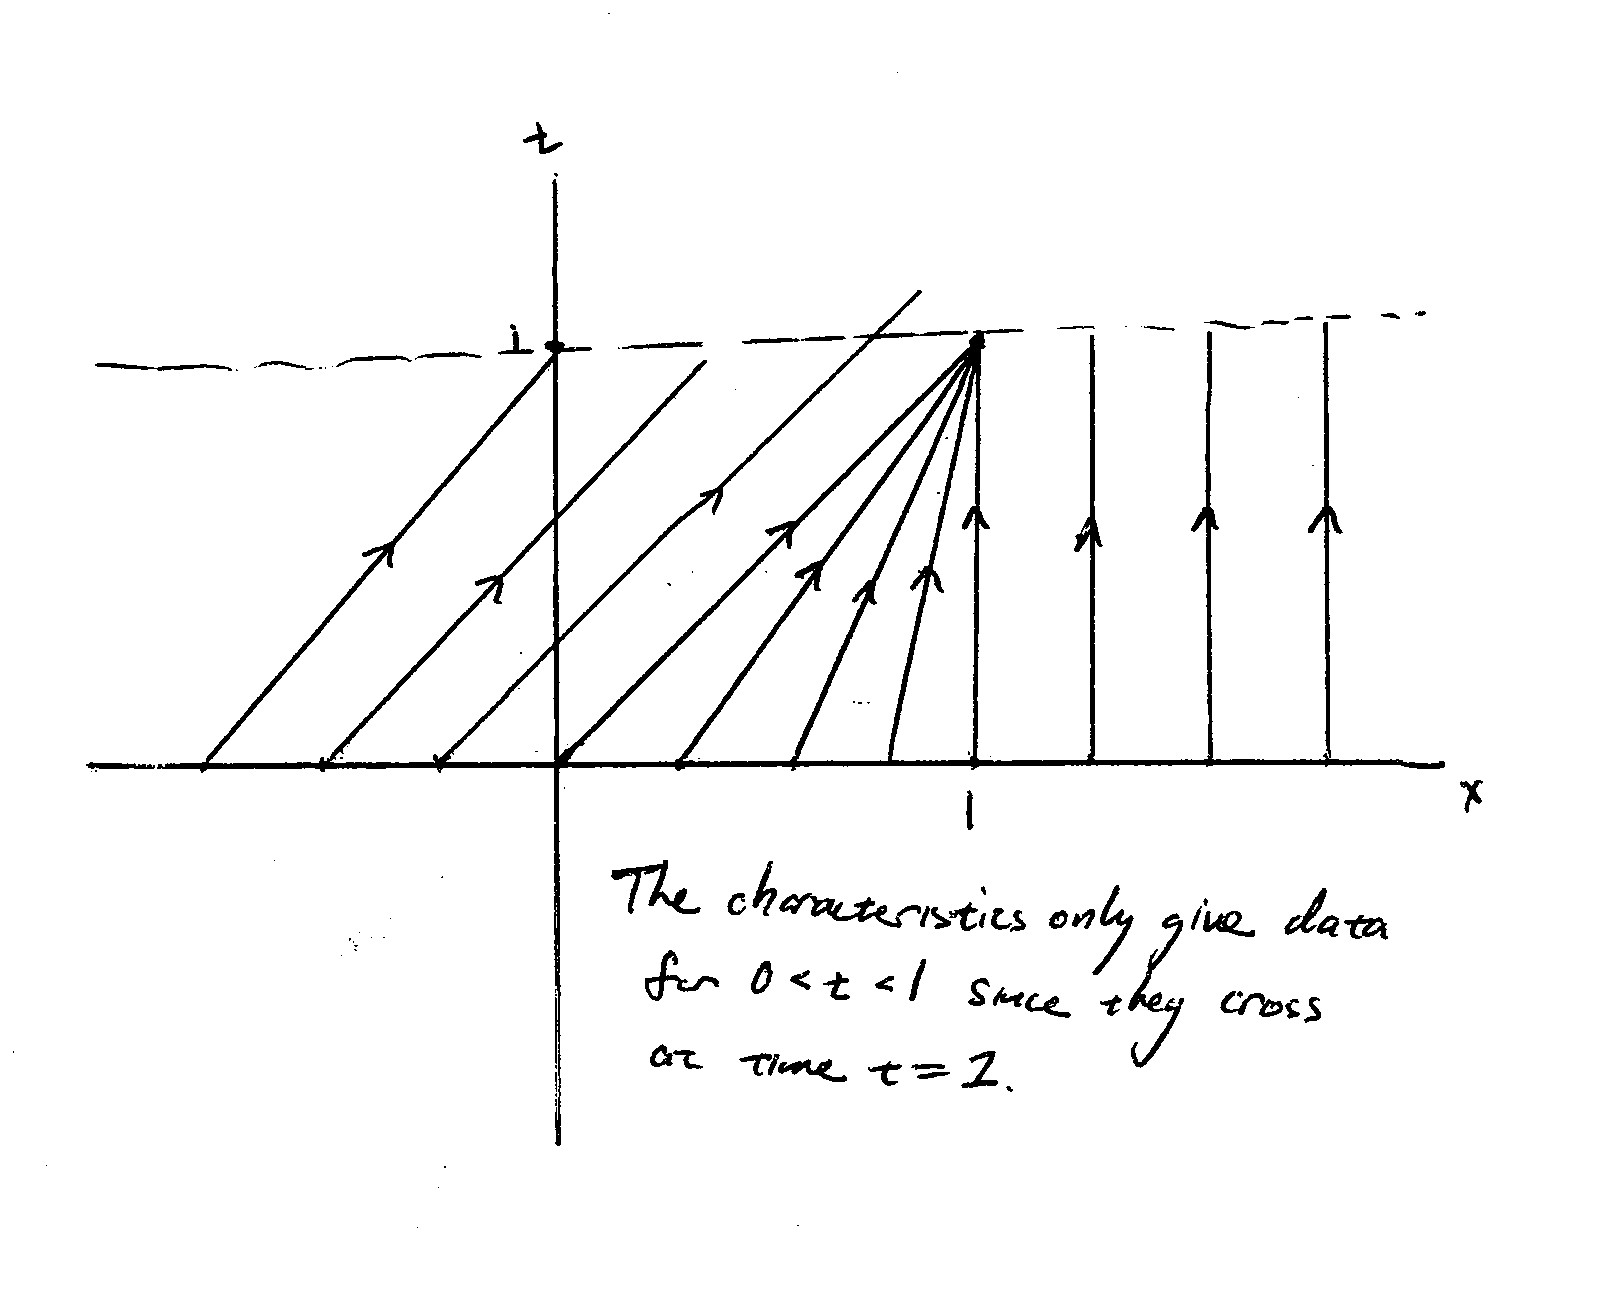
\includegraphics[scale=0.8]{./_Figures/F08Q3.jpg}
\end{center}
The characteristics cross at time $t = 1$ and hence for $t < 1$, the solution is given by
\ba
u(x, t) = \begin{cases}
0 & \text{ if } x > 1\\
1 - \frac{x - t}{1 - t} = \frac{1 - x}{1 - t} & \text{ if } 0 < \frac{x - t}{1 - t} < 1 \text{ (which happens if and only if $t < x < 1$)}\\
1 & \text{ if } x - t < 0 \text{ (which happens if and only if $x < t$)}.
\end{cases}
\ea
Since the characteristics cross, now we compute the shock curve $x = s(t)$. We have
$f(u) = (1/2)u^2$ and
$$\dot{s}(t) = \frac{f(1) - f(0)}{1 - 0}\quad \text{ with }\quad s(1) = 1.$$
Thus $\dot{s}(t) = 1/2$, $s(1) = 1$ which implies $s(t) = (t + 1)/2$. Therefore for $t > 1$, the entropy solution is
\ba
u(x, t) = \begin{cases}
1 & \text{ if } x < \frac{1}{2}(t + 1)\\
0 & \text{ if } x > \frac{1}{2}(t + 1).
\end{cases}
\ea
\hq

\sub{Solution to Fall 2008, \#4}\label{f084}
There is a rigorous argument in Evans. We will proceed nonrigorously. Let $\eta = x - ct$. Then $u_t = u_{xx} + 1 - u^2$ becomes
$-cf' = f'' + 1 - f^2$. Writing this as a system gives that we need to analyze
\ba
x' &= y\\
y' &= -cy - 1 + x^2.
\ea
The stationary points are $(1, 0)$ and $(-1, 0)$.
The Jacobian is $J(x, y) = \smat{0}{1}{2x}{-c}$ and hence $J(1, 0) = \smat{0}{1}{2}{-c}$ and $J(-1, 0) = \smat{0}{1}{-2}{-c}$.
\begin{enumerate}[$(i)$]
\item $J(1, 0) = \smat{0}{1}{2}{-c}$: This matrix has eigenvalues $\ld = \frac{-c \pm \sqrt{c^2 + 8}}{2}$ and hence is a saddle
for all $c > 0$.
\item $J(-1, 0) = \smat{0}{1}{-2}{-c}$: This matrix has eigenvalues $\ld = \frac{-c \pm \sqrt{c^2 - 8}}{2}$ and hence
is a sink node if $c > 2\sqrt{2}$, a stable spiral if $c < 2\sqrt{2}$, and an improper node if $c = 2\sqrt{2}$.
\end{enumerate}
If $c < 2\sqrt{2}$, then $(-1, 0)$ is a spiral and so that there are times for which $y > 0$.
Since $y = x'$, we have that $x$ is not monotonically decreasing when $c < 2\sqrt{2}$. Translating this back to the problem,
we have shown that $f$ is not monotonically decreasing when $c < 2\sqrt{2}$.

Let $\ld_{\pm} := \frac{-c \pm \sqrt{c^2 + 8}}{2}$. Note that $\smat{0}{1}{2}{-c}\svt{a}{b} = \ld_{\pm}\svt{a}{b}$ implies
$b = \ld_{\pm}a$. Thus the eigenvectors for this eigenvalue is $$\vct{1}{\ld_{\pm}} = \vct{1}{\frac{-c \pm \sqrt{c^2 + 8}}{2}}$$
and so locally near $(1, 0)$, the phase plane looks like
\begin{center}
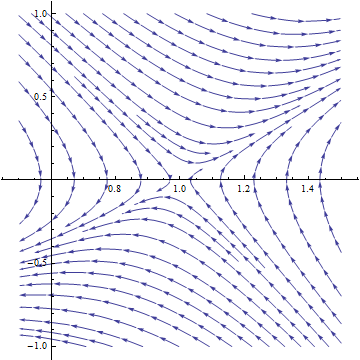
\includegraphics[scale=0.75]{./_Figures/F08Q4.png}
\end{center}
Since $(-1, 0)$ is either a stable spiral or a sink, then there exists a unique $f$ such that $\lim_{x \rightarrow -\infty}f(x) = 1$
and $\lim_{x \rightarrow \infty}f(x) = -1$.
\hq

\sub{Solution to Fall 2008, \#5}\label{f085}
We want to show that
\ba
\int_{\R^3}-\frac{1}{4\pi}\int_{\R^3}\frac{f(y)}{|x - y|}\, dy \lap \phi(x)\, dx = \int_{\R^3}f(x)\phi(x)\, dx.
\ea
By Fubini's Theorem,
\ba
\int_{\R^3}f(y)\int_{\R^3}-\frac{1}{4\pi|x - y|}\lap \phi(x)\, dx\, dy = \int_{\R^3}f(y)\phi(y)\, dy.
\ea
Thus it suffices to prove that for each $x \in \R^3$,
$$\phi(x) = \int_{\R^3}\lap_{y}\phi(y)(-\frac{1}{4\pi\abn{y - x}})\, dy.$$
We have
\ba
\int_{\R^3}\lap_{y}\phi(y)(-&\frac{1}{4\pi\abn{y - x}})\, dy = \int_{\R^3}(-\lap_{y}\phi)(x - y)\frac{1}{4\pi\abn{y}}\, dy\\
&=\int_{B(0, \vep)}(-\lap_{y}\phi)(x - y)\frac{1}{4\pi\abn{y}}\, dy + \int_{\R^3\bs B(0, \vep)}(-\lap_{y}\phi)(x - y)\frac{1}{4\pi\abn{y}}\, dy.
\ea
Observe that
\ba
\abb{\int_{B(0, \vep)}(-\lap_{y}\phi)(x - y)\frac{1}{4\pi\abn{y}}\, dy} &\lsm \nms{\lap \phi}_{L^{\infty}}\int_{B(0, \vep)}\frac{1}{\abn{y}}\, dy\\
 &\lsm \abn{\lap\phi}_{L^{\infty}}\int_{0}^{\vep}\frac{1}{r}r^2\, dr \lsm \nms{\lap\phi}_{L^{\infty}}\vep^{2} \rightarrow 0
\ea
as $\vep \rightarrow 0$
and with $\kap(y) = -\frac{1}{4\pi\abn{y}}$,
\ba
\int_{\R^3\bs B(0, \vep)}&(-\lap_{y}\phi)(x - y)\frac{1}{4\pi\abn{y}}\, dy = \int_{\R^3\bs B(0, \vep)}\lap_{y}\phi(x - y)\kap(y)\, dy\\
&=\int_{\R^3 \bs B(0, \vep)}\phi(x - y)\lap\kap(y)\, dy + \int_{\pr(\R^3\bs B(0, \vep))}-\phi(x - y)\frac{\pr\kap}{\pr \nu} + \kap(y)\frac{\pr\phi}{\pr\nu}(x - y)\, d\sigma.
\ea
Since $\lap\kap = 0$ on $\R^3 \bs B(0, \vep)$ and
\ba
\int_{\pr(\R^3 \bs B(0, \vep))}\kap(y)\frac{\pr\phi}{\pr\nu}(x - y)\, d\sigma \lsm \nms{\del \phi}_{L^{\infty}}\int_{\pr B(0, \vep)}\frac{1}{\abn{y}}\, d\sigma \lsm \vep\nms{\del \phi}_{L^{\infty}} \rightarrow 0
\ea
as $\vep \rightarrow \infty$ we have
\ba
\int_{\R^3}\lap_{y}\phi(y)(-\frac{1}{4\pi\abn{y - x}})\, dy = \lim_{\vep \rightarrow 0}\int_{\pr(\R^3\bs B(0, \vep))}\phi(x - y)\frac{\pr \kap}{\pr\nu}\, d\sigma.
\ea
Since $\del \kap(y) = \frac{1}{4\pi}\frac{y}{\abn{y}^3}$ and $\nu = -y/\abn{y}$, we have
$$\frac{\pr \kap}{\pr\nu} = -\frac{1}{4\pi}\frac{\abn{y}^{2}}{\abn{y}^4} = -\frac{1}{4\pi}\frac{1}{\abn{y}^2}.$$
Then
\ba
\int_{\pr(\R^3\bs B(0, \vep))}-\phi(x - y)\frac{\pr \kap}{\pr \nu}\, d\sigma &= \frac{1}{4\pi\vep^2}\int_{\pr B(0, \vep)}\phi(x - y)\, d\sigma(y)\\
 &= \frac{1}{4\pi\vep^2}\int_{\pr B(x, \vep)}\phi(y)\, d\sigma(y) \rightarrow \phi(x)
\ea
as $\vep \rightarrow 0$. This shows that
$$\phi(x) = -\frac{1}{4\pi}\int_{\R^3}\frac{\lap \phi(y)}{\abn{x - y}}\, dy.$$

\begin{rem}
Alternatively, $-\frac{1}{4\pi\abn{x}}$ is the fundamental solution of the Laplacian.
Let $v(x) := -\frac{1}{4\pi}\int_{\R^3}\frac{\lap \phi(y)}{\abn{x - y}}\, dy$. Then
$\lap(v - \phi) = 0$ in $\R^3$. Since $\phi, v \rightarrow 0$ as $\abn{x} \rightarrow \infty$,
it follows that $v = \phi$. \hq
\end{rem}

\sub{Solution to Fall 2008, \#7}\label{f087}
We have
$$\int_{0}^{1}uu_{xxt} + uu_{xx} - u^{4}\, dx = 0$$
and hence
$$-\int_{0}^{1}u_{x}u_{xt}\, dx - \int_{0}^{1}u_{x}^{2}\, dx - \int_{0}^{1}u^{4}\, dx = 0.$$
Let $$w(t) := \int_{0}^{1}u_{x}^{2}\, dx.$$
Then $w'(t) = \int_{0}^{1}2u_{x}u_{xt}\, dx$. Thus
$$-\frac{1}{2}w'(t) - w(t) = \int_{0}^{1}u^{4}\, dx \geq 0$$
which implies
$$\frac{1}{2}w'(t) + w(t) \leq 0$$
and hence
$$(e^{2t}w(t))' \leq 0.$$
Thus $e^{2t}w(t)$ is monotonically decreasing. Then
$e^{2t}w(t) \leq w(0)$ which after rearranging gives
$$w(t) \leq e^{-2t}w(0).$$
Since
$$w(0) = \int_{0}^{1}(u_{x})^{2}(x, 0)\, dx = \int_{0}^{1}(2x - 1)^{2}\, dx = \frac{1}{3},$$
we have
$$0 \leq w(t) \leq \frac{1}{3}e^{-2t}.$$
Thus
\ba
\abn{u(y, t)} = \abb{\int_{0}^{y}u_{x}(x, t)\, dx} \leq \bigg(\int_{0}^{1}\abn{u_{x}(x, t)}^{2}\, dx\bigg)^{1/2} \leq \frac{e^{-t}}{\sqrt{3}} \rightarrow 0
\ea
as $t \rightarrow \infty$.
\hq

\sub{Solution to Fall 2008, \#8}\label{f088}
By Sturm-Liouville theory, the smallest $\ld$ for the eigenvalue problem $$u'' - q(x)u = -\ld u$$
is given by
$$\ld = \min_{u: u'(0) = u'(1) = 0}\frac{\ips{u, Lu}}{\ips{u, u}}.$$
Pick a smooth compactly supported function $u_{0}$ such that
$u_{0}'(0) = u_{0}'(1) = 0$ and $\int_{0}^{1}qu_{0}\, dx \neq 0$. Consider
$\ips{u_{0} + c, L(u_{0} + c)}$ for some $c$ to be chosen later. We have
\ba
\ips{u_{0} + c, &L(u_{0} + c)} = \ips{u_{0} + c, Lu_{0} + Lc} = \ips{u_{0}, Lu_{0}} + \ips{u_{0}, Lc} + c\ips{1, Lu_{0}} + \ips{c, Lc}\\
& = \ips{u_{0}, Lu_{0}} + c\int_{0}^{1}u_{0}q\, dx + c\int_{0}^{1}-u_{0}'' + qu_{0}\, dx = \ips{u_{0}, Lu_{0}} + 2c\int_{0}^{1}u_{0}q\, dx.
\ea
Now choose $c$ such that $\ips{u_{0}, Lu_{0}} + 2c\int_{0}^{1}u_{0}q\, dx < 0$. Then with this choice of $c$,
\ba
\ld = \min_{u: u'(0) = u'(1) = 0}\frac{\ips{u, Lu}}{\ips{u, u}} \leq \frac{\ips{u_{0} + c, L(u_{0} + c)}}{\ips{u_{0} + c, u_{0} + c}} < 0.
\ea
\hq
